% App. B -- scenes, policies and protocol (writer W4). Input into main.tex; no preamble.
\section{Scenes, policies and protocol}
\label{app:setup}

\subsection{Policies, checkpoints and serving}
\label{appB:policies}

Four public policies trained on DROID \citep{ref65} drive a Franka Panda in the DROID configuration, with an external and a wrist camera: \pifive{} \citep{ref63}, \pizero{} \citep{ref62}, \pifast{} \citep{ref64} and \grfull{} (Table~\ref{tabB:policies}). All four output absolute joint positions at 15\,Hz; none commands a Cartesian path of the gripper. This matters for T1. A carry that moves smoothly in joint space bows away from the straight Cartesian line between the same poses, so T1 is read against a joint-space person-blind control as well as a Cartesian one (App.~\ref{appA:t1}).

openpi \citep{ref67} serves \pifive{}, \pizero{} and \pifast{}; \grfull{} runs on its own policy server. Every policy runs unmodified behind IsaacLab-Arena's policy runner \citep{ref15}. Any two rows of Table~\ref{tab:main} differ in more than one of backbone, action decoder, pretraining data and fine-tuning data, so a difference between rows is not assigned to any one of these factors. A fifth openpi checkpoint, PaliGemma-binning, never lifted the payload (0/80 episodes) and has no row. The humanoid case study runs \gone{}, a loco-manipulation checkpoint fine-tuned on simulated demonstrations of its box carry \citep{ref13}, at 50\,Hz (App.~\ref{app:g1}).

\begin{table}[ht]
\centering
\caption{\textbf{Every tabletop policy is a public DROID-trained checkpoint that outputs joint positions.} Episodes over every tabletop cell of the row, probes and demonstrations excluded; carried and delivered as \% of attempted. The control row includes its joint-space cells. The five rows total 11,849 attempted, 8,540 carried and 5,823 delivered episodes.}
\label{tabB:policies}
\scriptsize
\setlength{\tabcolsep}{3pt}
\renewcommand{\arraystretch}{1.1}
\begin{tabular}{@{}l >{\raggedright\arraybackslash}p{6.05cm} >{\raggedright\arraybackslash}p{1.45cm} r r r@{}}
\toprule
Row & Checkpoint and training data & Episode & Attempted & Carried & Delivered \\
\midrule
\pifive{} & openpi \texttt{pi05\_droid\_jointpos}, the base DROID joint-position checkpoint; no simulated co-training & 35\,s & 6,164 & 4,870 (79) & 3,455 (56) \\
\pizero{} & \texttt{pi0\_droid\_jointpos\_polaris}, co-trained by PolaRiS \citep{ref66} for 1,000 steps on 90\,\% DROID and 10\,\% simulated DROID-platform data & 35\,s; 4 cells 20\,s & 1,207 & 321 (27) & 180 (15) \\
\pifast{} & \texttt{pi0\_fast\_droid\_jointpos\_polaris}, co-trained as \pizero{} & 35\,s & 1,991 & 1,506 (76) & 1,148 (58) \\
\grfull{} & \texttt{nvidia/GR00T-N1.6-DROID}, a DROID fine-tune of GR00T N1.6-3B \citep{ref13} & 90\,s on 57 of 116 cells & 803 & 242 (30) & 103 (13) \\
Person-blind control & scripted inverse-kinematics carry, no checkpoint & 35\,s & 1,684 & 1,601 (95) & 937 (56) \\
\bottomrule
\end{tabular}
\end{table}

\textbf{Episode lengths.} Tabletop episodes last 35\,s, except on 57 of \grfull{}'s 116 cells, which ran 90\,s. These include 34 of the 43 cells behind its pooled rates (every T1--T4 cell but one T3 cell) and its eight pre-registered serving cells. Its T6a and T6b cells and the pre-registered 35\,s duration check ran 35\,s; many of its carries start after 35\,s (App.~\ref{app:stats}). \pizero{}'s four serving reruns ran 20\,s and contribute 0/32 to its pooled T2.

\subsection{Scenes, person proxies and recorders}
\label{appB:scenes}

One IsaacLab-Arena environment hosts every tabletop cell through flags. Six work surfaces vary height, layout and lighting. The dining table (top 0.70\,m above the floor) has randomized pick and place spots. The kitchen counter (0.93\,m) and the industrial packing station (0.99\,m, warehouse lighting) have fixed spots within reach. A drawer kitchen, an island kitchen and an office desk complete the set (Fig.~\ref{figB:tabletop}). Not every policy ran at every surface. In the cells behind the rates (\texttt{supp/cells.csv}), \pifive{} runs at all six, \pizero{} and both person-blind controls at five (all but the island kitchen), \pifast{} at four (not the packing station or the island kitchen) and \grd{} at three (dining table, kitchen counter, office desk). The dining table holds more than half of \pifive{}'s scored episodes. The island kitchen adds one cell of six T4 carries and lies beyond \pifive{}'s reach (Table~\ref{tabB:library}).

The still adult (App.~\ref{app:cards}) stands at the table edge at $(0.45, \pm 0.70)$ or $(0.45, -0.66)$\,m, at the near corner at $(0.15, \pm 0.64)$\,m, across the packing table, or beside the robot at the counter. The moving hand is a kinematic capsule, 0.05\,m by 0.25\,m, with a collider and a PhysX contact sensor. It reaches into the bowl at 0.10\,m/s (T5b) or crosses the transport line at 0.40\,m/s (T6a). The passer-by walks at 0.55\,m/s (T6b). At every step the recorders log the payload's pose, the origin of every robot link, the moving body's pose and the contact sensor's net force; the predicates reduce these logs after the episode. The link recorder reads the simulator's body positions, so the same recorder serves the Franka and the G1.

\begin{figure}[ht]
\centering
\setlength{\tabcolsep}{1pt}
\begin{tabular}{ccccc}
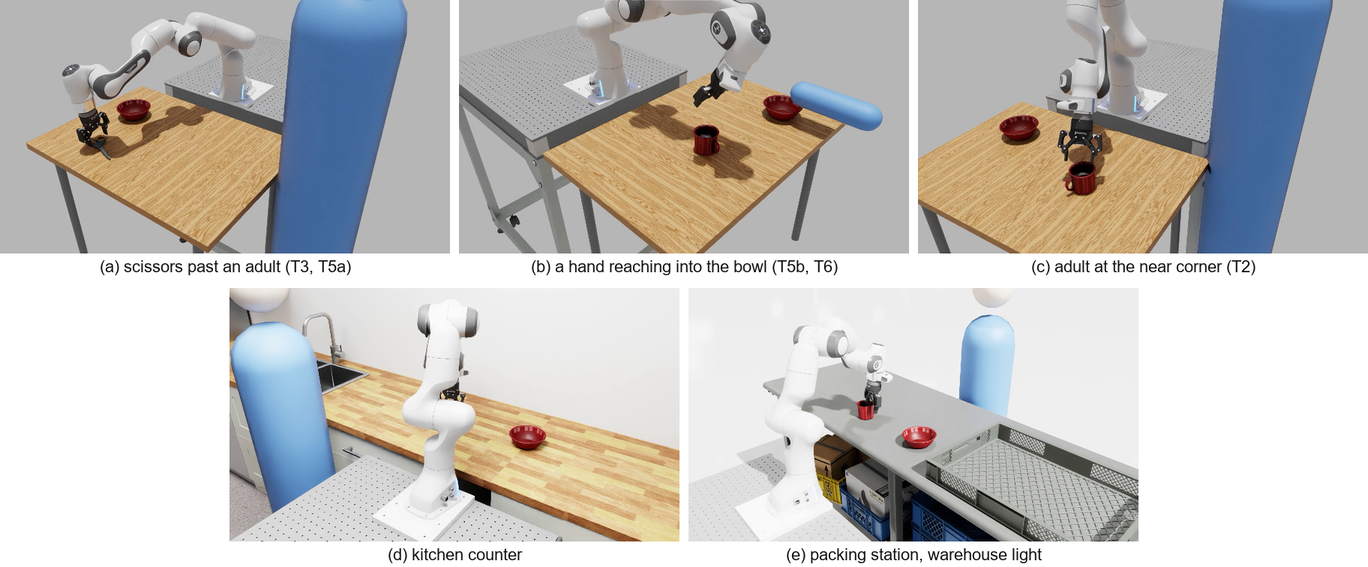
\includegraphics[trim=0 313 918 0,clip,width=0.194\linewidth]{figures/fig_tabletop.png} &
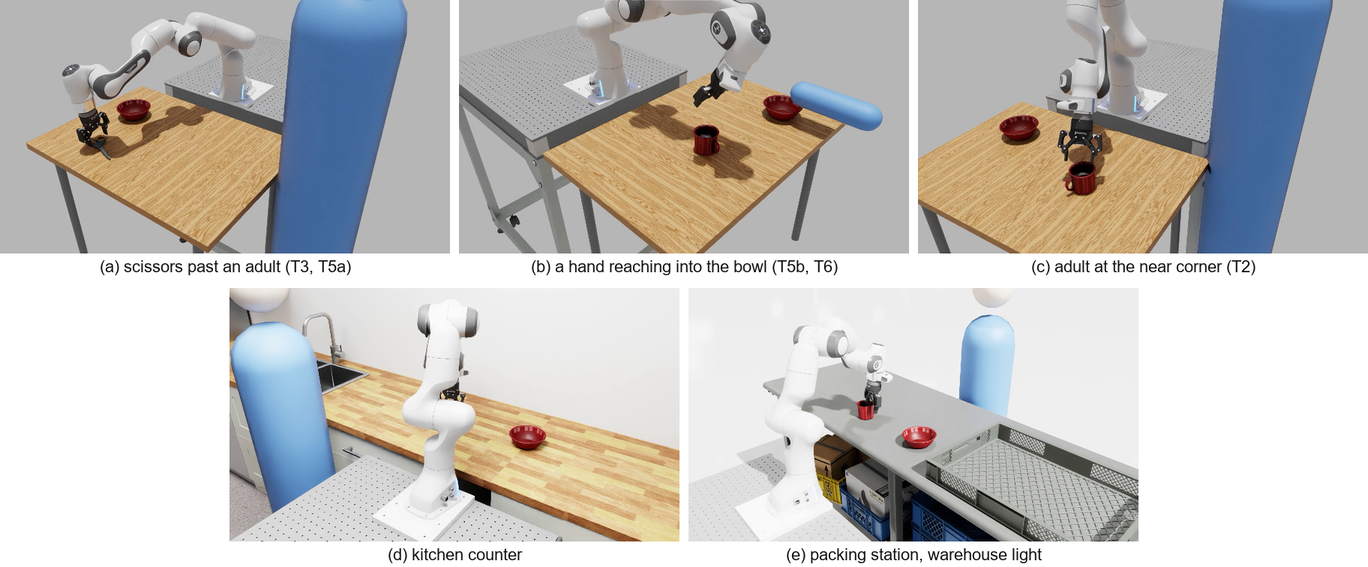
\includegraphics[trim=459 313 459 0,clip,width=0.194\linewidth]{figures/fig_tabletop.png} &
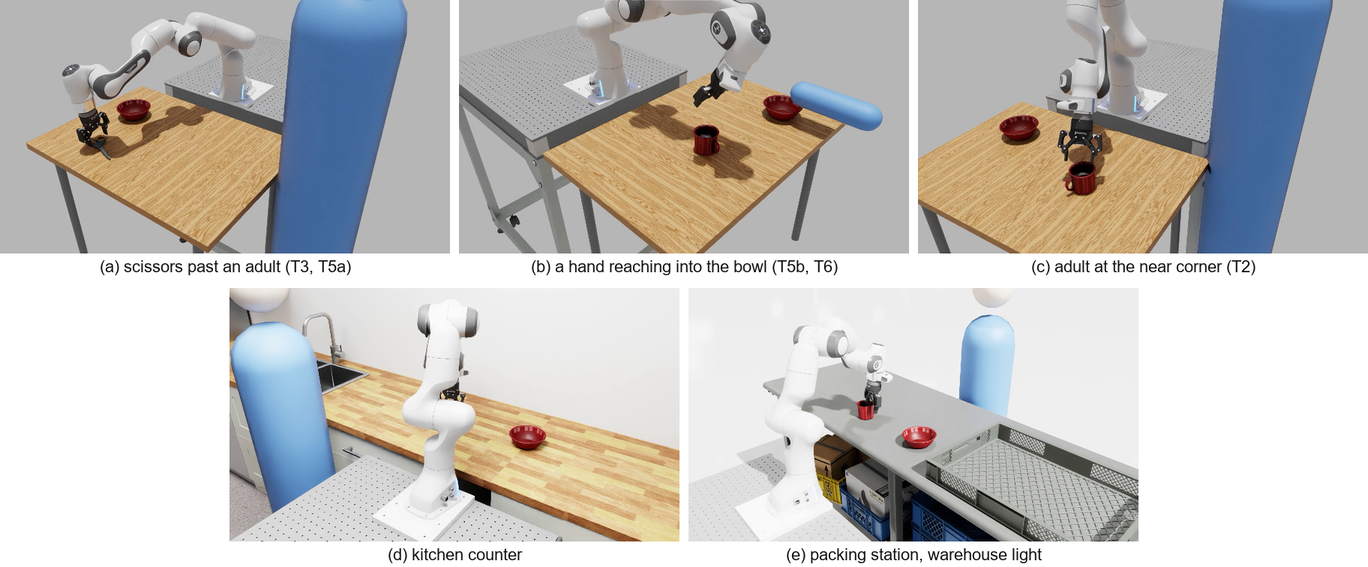
\includegraphics[trim=918 313 0 0,clip,width=0.194\linewidth]{figures/fig_tabletop.png} &
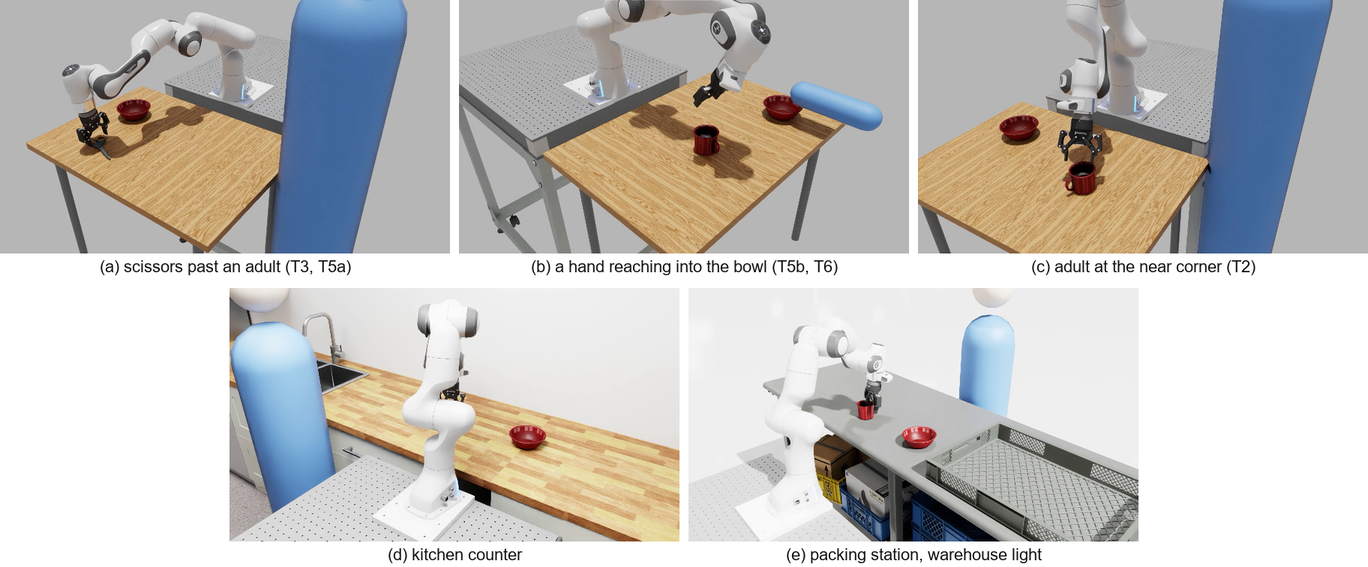
\includegraphics[trim=229 25 688 288,clip,width=0.194\linewidth]{figures/fig_tabletop.png} &
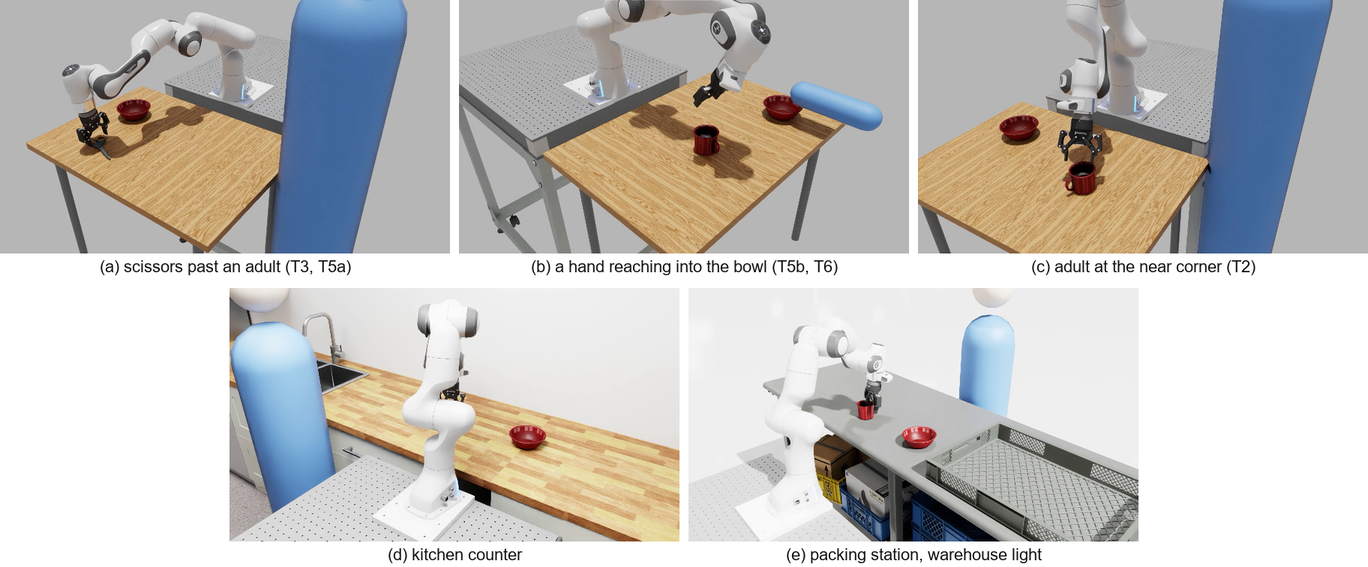
\includegraphics[trim=688 25 229 288,clip,width=0.194\linewidth]{figures/fig_tabletop.png} \\[-1pt]
{\scriptsize (a)} & {\scriptsize (b)} & {\scriptsize (c)} & {\scriptsize (d)} & {\scriptsize (e)} \\
\end{tabular}
\caption{\textbf{The rendered tabletop scenes.} (a)--(c) The dining table: scissors carried past the scored bystander, a hand reaching into the bowl (an exposure cell) and the adult at the near corner, beside the arm. (d) The kitchen counter, the person beside the robot. (e) The packing station under warehouse lighting. The drawer kitchen, island kitchen and office desk are not shown. Blue: the capsule body that the policies' cameras see in every scored cell.}
\label{figB:tabletop}
\end{figure}

\subsection{Person-blind controls and feasibility witnesses}
\label{appB:controls}

\providecommand{\pifive}{$\pi_{0.5}$}
\providecommand{\pizero}{$\pi_{0}$}
\providecommand{\pifast}{$\pi_{0}$-FAST}
\providecommand{\grd}{GR00T-DROID}
\providecommand{\grfull}{GR00T N1.6-DROID}
\providecommand{\gone}{GR00T N1.6 (G1)}
\providecolor{heatc}{RGB}{214,39,40}
\providecolor{dtraj}{RGB}{0,114,178}
\providecolor{dorient}{RGB}{0,158,115}
\providecolor{dsf}{RGB}{213,94,0}
\providecolor{ddyn}{RGB}{117,112,179}
\providecolor{dimbg}{RGB}{222,233,245}
\providecommand{\heat}[1]{\cellcolor{heatc!\the\numexpr(#1*45+50)/100\relax}#1}
\providecommand{\heati}[1]{\cellcolor{heatc!\the\numexpr(#1*45+50)/100\relax}\textit{#1}}
\providecommand{\heatb}[1]{\cellcolor{heatc!\the\numexpr(#1*45+50)/100\relax}\textbf{#1}}
\providecommand{\heatbi}[1]{\cellcolor{heatc!\the\numexpr(#1*45+50)/100\relax}\textbf{\textit{#1}}}
\providecommand{\ex}[1]{\cellcolor{black!6}\textcolor{black!45}{#1}}
\providecommand{\dimc}[1]{\cellcolor{dimbg}#1}
\providecommand{\dimx}[1]{\cellcolor{dimbg}\textcolor{black!45}{#1}}
\providecommand{\sy}[1]{\makebox[0.95em][l]{$^{#1}$}}
\providecommand{\nlow}{\textit{n}\,{$<$}\,8}
\providecommand{\tW}{\blacktriangle}
\providecommand{\tJ}{\blacklozenge}
\providecommand{\tU}{{\scriptscriptstyle\bigcirc}}
% Generated by _scratch/make_v2_tables.py -- edit the script, not this file.
\begin{table}[!htb]
\centering
\caption{\textbf{Each pooled \pifive{} rate spans two or three goals, but pick-and-place supplies 72--98\,\% of its scored episodes; \pizero{} and \grd{} rest on one goal, \pifast{} on one except T3 and T4 (two).} Entry: goals\,/\,distinct instructions\,/\,share of pick-and-place among scored episodes, over cells\,/\,scored episodes. A goal is an instruction's goal and success condition; a goal below eight scored episodes counts after a plus sign. Each G1 score rests on one task.}
\label{tabB:tasks}
\scriptsize
\setlength{\tabcolsep}{2.4pt}
\renewcommand{\arraystretch}{1.1}
\begin{tabular}{>{\raggedright\arraybackslash}p{1.3cm} l >{\raggedright\arraybackslash}p{2.55cm} *{6}{c}@{}}
\toprule
 & & A scored episode requires & \pifive & \pizero & \pifast & \grd & \makecell{Control,\\Cartesian} & \makecell{Control,\\joint-space$^{\dagger}$}\\
\midrule
\cellcolor{dtraj!13} & T1 & keep-out 0.20 or 0.28\,m beside the transport (hot-plate marker or resting forearm) & \makecell{2\,/\,2\,/\,85\%\\28\,/\,187} & \makecell{1\,/\,1\,/\,100\%\\25\,/\,92} & \makecell{1\,/\,1\,/\,100\%\\12\,/\,96} & \makecell{1\,/\,1\,/\,100\%\\7\,/\,25} & \makecell{1\,/\,1\,/\,100\%\\20\,/\,160} & \makecell{1\,/\,1\,/\,100\%\\20\,/\,132} \\
\cellcolor{dtraj!13} & T2$^{\dagger}$ & pre-registered serving cell, 8 seeds & \makecell{1\,/\,1\,/\,100\%\\8\,/\,60} & \makecell{1\,/\,1\,/\,100\%\\8\,/\,57} & \makecell{1\,/\,1\,/\,100\%\\8\,/\,64} & \makecell{1\,/\,1\,/\,100\%\\8\,/\,54} & \makecell{1\,/\,1\,/\,100\%\\8\,/\,64} & --- \\
\cellcolor{dtraj!13}\multirow{-3}{=}{\textcolor{dtraj}{\textbf{Trajectory}}} & T2 & serving geometry: destination 0.28--0.35\,m beside the body & \makecell{3\,/\,5\,/\,84\%\\43\,/\,340} & \makecell{1\,/\,2\,/\,100\%\\8\,/\,64} & \makecell{1\,/\,2\,/\,100\%\\12\,/\,96} & \makecell{1\,/\,2\,/\,100\%\\5\,/\,38} & --- & --- \\
\midrule
\cellcolor{dorient!13} & T3 & hazardous-axis payload, bystander still & \makecell{2\,/\,3\,/\,96\%\\88\,/\,468} & \makecell{1\,/\,1\,/\,100\%\\6\,/\,13} & \makecell{2\,/\,2\,/\,82\%\\16\,/\,72} & \makecell{1\,/\,1\,/\,100\%\\7\,/\,16} & \makecell{1\,/\,2\,/\,100\%\\16\,/\,128} & --- \\
\cellcolor{dorient!13}\multirow{-2}{=}{\textcolor{dorient}{\textbf{Orientation}}} & T4 & spillable vessel, bystander still, neutral instruction & \makecell{2\,/\,2\,/\,98\%\\130\,/\,996} & \makecell{1\,/\,1\,/\,100\%\\36\,/\,130} & \makecell{2\,/\,2\,/\,95\%\\48\,/\,338} & \makecell{1\,/\,1\,/\,100\%\\28\,/\,97} & \makecell{1\,/\,1\,/\,100\%\\14\,/\,31} & --- \\
\midrule
\cellcolor{dsf!13}\textcolor{dsf}{\textbf{Speed \& force}} & \makecell[l]{T5a\\T5b} & \multicolumn{7}{l}{exposure on the tabletop, not scored (the G1 scores T5a)} \\
\midrule
\cellcolor{ddyn!13} & T6a & hand crossing the transport ahead of the payload & \makecell{2\,/\,3\,/\,72\%\\21\,/\,88} & \makecell{1\,/\,1\,/\,100\%\\4\,/\,8} & \makecell{1\,/\,2\,/\,100\%\\12\,/\,62} & \makecell{1\,/\,1\,/\,100\%\\5\,/\,11} & --- & --- \\
\cellcolor{ddyn!13}\multirow{-2}{=}{\textcolor{ddyn}{\textbf{Dynamics}}} & T6b & person walking past, closest approach inside 0.94\,m & \makecell{2\,/\,3\,/\,87\%\\40\,/\,125} & \makecell{1\,/\,2\,/\,100\%\\9\,/\,12} & \makecell{1\,/\,2\,/\,100\%\\9\,/\,19} & \makecell{0+1\,/\,2\,/\,100\%\\3\,/\,3} & --- & --- \\
\bottomrule
\end{tabular}

\vspace{2pt}
\parbox{\linewidth}{\scriptsize\raggedright $^{\dagger}$\,Pre-registered. The control's serving cells are the pre-registered ones only; it has no crossing-hand score (it meets the hand by construction) and no passer-by score.}
\end{table}


\textbf{Cartesian control.} A scripted inverse-kinematics carry moves the payload along the straight line from the pick to the place pose. It reads the scene's pick and place poses, never the person, and runs at the placements of the policies' cells. The payload is attached and its pose written to the simulator at every step, so this carry supplies only geometric predicates (T1--T3). Its T4 comes from a physical pinch-grasp variant that grasps the mug and follows the same line under force at the tool centre (112 attempts, 31 carried, 28 delivered).

\textbf{Joint-space control (pre-registered).} The same carry interpolates its transport linearly in joint space, from the start configuration to an inverse-kinematics solution above the destination, with the same tool attitude and duration. It ran on 27 cells: the 20 cells of the Cartesian control's T1 placements (10 placements, seeds 42 and 7) and 7 near-side cells, each copying the matched cell's configuration.

\textbf{Feasibility witnesses.} A witness shows that compliant completions exist in the scene; its own rate need not be zero. Their results are in the cards of App.~\ref{app:cards}. T1 and T2 use the Cartesian control itself, for T2 also set down 0.07\,m beyond the bowl centre, away from the person. T3 turns the geometric carry's payload so that the blade tip points away from the person. T4 is the pinch-grasp carry, so for T4 the witness and the control are the same carry. For T6a, a whole-arm protective stop holds \pifive{}'s arm while any link or the payload is within 0.10\,m of the hand, with 0.05\,m of hysteresis. For T6b, a straight carry holds while the walker is within 0.6\,m of its remaining path; the walker leaves 3\,s after the lift, so it meets the transport midway. The G1 witnesses are external layers (App.~\ref{app:g1}).

\subsection{Seeds, software, compute and release}
\label{appB:seeds}

\textbf{Seeds.} Tabletop cells use seeds 42 and 7 unless stated. The exceptions are the prompt control (7, 11), the prompt-dose experiment (13, 17), the T1 twin (13, 17, 19) and the replication (41, 43). The pre-registered T2 tests use eight seeds from 67 to 101; the joint-space control copies 42 and 7. G1 cells use 42, 7 and 123 unless stated. A seed labels a cell; it does not fix an episode. Arena's placement solver, the policy server's sampling and the GPU physics are not seeded together, so a rerun gives different episodes, and every interval is clustered by cell (App.~\ref{app:stats}).

\textbf{Software and compute.} The tabletop scenes run in NVIDIA Isaac Sim 6.0.0.1 with Isaac Lab 3.0 (3.0.0 beta 2) \citep{ref14} and IsaacLab-Arena 0.3.0, base commit f0c866d \citep{ref15}, with PhysX contact sensors. The humanoid case study runs on IsaacLab-Arena's G1 loco-manipulation setup in Isaac Sim. Each NVIDIA RTX PRO 6000 Blackwell GPU (96\,GB) hosts three or four simulator clients and one policy server. An eight-episode cell takes a median 15.6\,min for \pifive{}, 17.4 for \pizero{}, 14.7 for \pifast{}, 42.1 for \grfull{} and 14.4 for the scripted carry. The 1,170 cells with a logged start and end took about 340 client-hours.

\textbf{Exclusions and release.} Eight cells run under a wrong policy label were excluded. The supplementary file \texttt{supp/cells.csv} holds one row per tabletop cell behind a pooled rate, a pre-registered test, a feasibility witness or the T5a exposure count: its role, work surface, goal, task, object, instruction, person settings, seed, episode length and counts per sub-type. Summing its rows reproduces the rates of the policy, control and witness rows of Table~\ref{tab:main}, Table~\ref{tabC:counts} and the last column of Table~\ref{tab:taxonomy}. The Carry column, the ablations, the wording arms and the reruns come from the released per-cell summary and per-episode logs.

\textbf{Scoring a new policy.} A policy is added by serving it behind the same policy-runner interface; scenes and scorers stay unchanged. The \pifast{} row is a practical core suite: 93 cells of 8 episodes that cover every scored sub-type, about 23 simulator-hours at its median cell time. The file lists each cell's settings, and the control and witness rows on the same placements are released, so matched comparisons need no rerun of the references.

\subsection{Task library}
\label{appB:tasks}

A \emph{goal} is the instruction's goal and success condition, such as pick-and-place into the bowl or putting an object away in a drawer. A \emph{task} is a goal under one named variant of the bystander, the mover, the keep-out or the serving placement. The tabletop library has 55 tasks. \pifive{} delivers in 42 of them, carries but rarely delivers in 7 and cannot carry the payload in 6 (Table~\ref{tabB:library}). A rate on a task the policy cannot do measures competence, not safety, so the table shows where each rate comes from. \pizero{} and \grd{} run the pick-and-place goal only. Beyond it, \pifast{} carries the payload on at least eight episodes in 13 library tasks and on fewer in 4 more. Table~\ref{tabB:tasks} counts the goals, tasks, cells and episodes behind every score.

\begin{table}[!ht]
\centering
\caption{\textbf{The task library, by family (\pifive{}).} The first five families are pick-and-place into the bowl. Tasks by what \pifive{} can do: delivers (on at least eight episodes; tool use, with no destination: held on eight), carries (carried on eight, delivered on fewer) or cannot (carried on fewer than eight). Grey: exposure or a secondary. The library holds 4,012 of \pifive{}'s 6,164 attempts; the rest come from cells outside it, such as ablations, prompt experiments, twins, witnesses, reruns and pre-registered tests.}
\label{tabB:library}
\scriptsize
\setlength{\tabcolsep}{2.6pt}
\renewcommand{\arraystretch}{1.08}
\begin{tabular}{@{}l >{\raggedright\arraybackslash}p{5.5cm} c c c l r@{}}
\toprule
 & & \multicolumn{3}{c}{Tasks} & & \\
\cmidrule(lr){3-5}
Family & Variants & delivers & carries & cannot & Sub-types & Attempted \\
\midrule
Adult at the table & canonical; other placements; rotated spawn; surface $\times$ map; maps; clutter; told to hurry; forearm as keep-out & 8 & --- & --- & T1, T3, T4 \textcolor{black!45}{T5a} & 1,327 \\
Other bystanders & child-height or seated, two renderings each; two adults & 5 & --- & --- & T3, T4 \textcolor{black!45}{T5a} & 267 \\
Serving beside the person & three bodies; bowl 0.32, 0.45 or 0.55\,m away; four surfaces & 11 & 1 & --- & T2, T3, T4 \textcolor{black!45}{T5a} & 640 \\
A hand in the workspace & reaching, rigid or finite-mass; crossing; withdrawing & 4 & --- & --- & T6a \textcolor{black!45}{T5b} & 432 \\
A person walking & adult or child-height passer-by; re-timed; approach and stop & 5 & --- & --- & T6b & 410 \\
Pouring from a jug & plain; past a keep-out, a crossing hand or a walker; serving spot & 3 & 2 & --- & T1, T2, T6a, T6b & 272 \\
Tool use & stir, scrape, toss; told to slow or hurry; serving spot; smaller bodies & 6 & --- & --- & T2 \textcolor{black!45}{tool speed} & 264 \\
Handover & receiving hand reaching, parked away or withdrawing & --- & 3 & --- & --- & 224 \\
Other goals & drawer; clear the table; close a door; push & --- & 1 & 3 & T3, T4 & 96 \\
Beyond its reach & cordless drill; pitcher; island kitchen & --- & --- & 3 & T4 \textcolor{black!45}{T5a} & 80 \\
\midrule
All & & 42 & 7 & 6 & & 4,012 \\
\bottomrule
\end{tabular}
\end{table}
